The GWT Model simulates three-dimensional transport of a single solute species in flowing groundwater \citep{modflow6gwt}.  The GWT Model solves the solute transport equation using numerical methods and a generalized control-volume finite-difference approach, which can be used with regular MODFLOW grids (DIS Package) or with unstructured grids (DISV and DISU Packages).  The GWT Model is designed to work with most of the new capabilities released with the GWF Model, including the Newton flow formulation, unstructured grids, advanced packages, and the movement of water between packages.  The GWF and GWT Models operate simultaneously during a \mf simulation to represent coupled groundwater flow and solute transport.  The GWT Model can also run separately from a GWF Model by reading the heads and flows saved by a previously run GWF Model.  The GWT model is also capable of working with the flows from another groundwater flow model, as long as the flows from that model can be written in the correct form to flow and head files.  

The purpose of the GWT Model is to calculate changes in solute concentration in both space and time.  Solute concentrations within an aquifer can change in response to multiple solute transport processes.  These processes include (1) advective transport of solute with flowing groundwater, (2) the combined hydrodynamic dispersion processes of velocity-dependent mechanical dispersion and chemical diffusion, (3) sorption of solutes by the aquifer matrix either by adsorption to individual solid grains or by absorption into solid grains, (4) transfer of solute into very low permeability aquifer material (called an immobile domain) where it can be stored and later released, (5) first- or zero-order solute decay or production in response to chemical or biological reactions, (6) mixing with fluids from groundwater sources and sinks, and (7) direct addition of solute mass.

With the present implementation, there can be multiple domains and multiple phases.  There is a single mobile domain, which normally consists of flowing groundwater, and there can be one or more immobile domains.  The GWT Model simulates the dissolved phase of chemical constituents in both the mobile and immobile domains.  The dissolved phase is also referred to in this report as the aqueous phase.  If sorption is represented, then the GWT Model also simulates the solid phase of the chemical constituent in both the mobile and immobile domains.  The dissolved and solid phases of the chemical constituent are tracked in the different domains by the GWT Model and can be reported as output as requested by the user.

This section describes the data files for a \mf Groundwater Transport (GWT) Model.  A GWT Model is added to the simulation by including a GWT entry in the MODELS block of the simulation name file.  There are three types of spatial discretization approaches that can be used with the GWT Model: DIS, DISV, and DISU.  The input instructions for these three packages are not described here in this section on GWT Model input; input instructions for these three packages are described in the section on GWF Model input.

The GWT Model is designed to permit input to be gathered, as it is needed, from many different files.  Likewise, results from the model calculations can be written to a number of output files. The GWT Model Listing File is a key file to which the GWT model output is written.  As \mf runs, information about the GWT Model is written to the GWT Model Listing File, including much of the input data (as a record of the simulation) and calculated results.  Details about the files used by each package are provided in this section on the GWT Model Instructions.

The GWT Model reads a file called the Name File, which specifies most of the files that will be used in a simulation. Several files are always required whereas other files are optional depending on the simulation. The Output Control Package receives instructions from the user to control the amount and frequency of output.  Details about the Name File and the Output Control Package are described in this section.

For the GWT Model, ``flows'' (unless stated otherwise) represent solute mass ``flow'' in mass per time, rather than groundwater flow.  

\subsection{Information for Existing Solute Transport Modelers}
The \mf GWT Model contains most of the functionality of MODFLOW-GWT, MT3DMS, MT3D-USGS and MODFLOW-USG.  The following list summarizes major differences between the GWT Model in \mf and previous MODFLOW-based solute transport programs.

\begin{enumerate}

\item The GWT Model simulates transport of a single chemical species; however, because \mf allows for multiple models of the same type to be included in a single simulation, multiple species can be represented by using multiple GWT Models.

\item For most simulations, the GWT Model needs groundwater flows for every cell in the model grid, for all boundary conditions, for all advanced package flow terms, and for other terms, such as the flow of water in or out of storage.  The GWT Model can access these flows in a GWF Model that is running in the same simulation as the GWT Model.  Alternatively, the GWT Model can read binary head and budget files created from a previous GWF Model simulation (provided these files contain all of the required information for all time steps); there is no specialized flow and transport link file \citep{zheng2001modflow} as there is for MT3D.  Details on these two different use cases are provided in the chapter on the FMI Package.

\item The GWT Model is based on a generalized control-volume finite-difference method, which means that solute transport can be simulated using regular MODFLOW grids consisting of layers, rows, and columns, or solute transport can be simulated using unstructured grids.

\item Advection can be simulated using central-in-space weighting, upstream weighting, or an implicit second-order TVD scheme.  The GWT model does not have the Method of Characteristics (particle-based approaches) or an explicit TVD scheme.  Consequently, the GWT Model may require a higher level of spatial discretization than other transport models that use higher order terms for advection dominated systems.  This can be an important limitation for some problems, which require the preservation of sharp solute fronts. 

\item Variable-density flow and transport can be simulated by including a GWF Model and a GWT Model in the same \mf simulation.  The Buoyancy Package should be activated for the GWF Model so that fluid density is calculated as a function of simulated concentration.  If more than one chemical species is represented then the Buoyancy Package allows the simulated concentration for each of them to be used in the density equation of state.   \cite{langevin2020hydraulic} describe the hydraulic-head formation that is implemented in the Buoyancy Package for variable-density groundwater flow and present the results from \mf variable-density simulations.  The variable-density capabilities available in \mf replicate and extend the capabilities available in SEAWAT to include the Newton flow formulation and unstructured grids, for example.  

\item The GWT Model has a Source and Sink Mixing (SSM) Package for representing the effects of GWF stress package inflows and outflows on simulated concentrations.  There are two ways in which users can assign concentrations to the individual features in these stress package.  The first way is to activate a concentration auxiliary variable in the corresponding GWF stress package.  In the SSM input file, the user provides the name of the auxiliary variable to be used for concentration.  The second way is to create a special SPC file, which contains user-assigned time-varying concentrations for stress package features.

\item The GWT model includes the MST and IST Packages.  These two package collectively comprise the capabilities of the MT3DMS Reactions Package.

\item The MST Package contains the linear, Freundlich, and Langmuir isotherms for representing sorption.  The IST Packages contains only the linear isotherm for representation of sorption. 

\item The GWT model was designed so that the user can specify as many immobile domains and necessary to represent observed contaminant transport patterns and solute breakthrough curves.  The effects of an immobile domain are represented using the Immobile Storage and Transfer (IST) Package, and the user can specify as many IST Packages as necessary.  

\item A GWT-GWT Exchange (introduced in version 6.3.0) can be used to tightly couple multiple transport models, as might be done in a nested grid configuration.  

\item There is no option to automatically run the GWT Model to steady state using a single time step.  This is an option available in MT3DMS \citep{zheng2010supplemental}.  Steady state conditions must be determined by running the transport model under transient conditions until concentrations stabilize.

\item The GWT Model described in this report is capable of simulating solute transport in the advanced stress packages of \mf, including the Lake, Streamflow Routing, Multi-Aquifer Well, Unsaturated Zone Transport Packages, and the Water Mover Package.  The present implementation simulates solute advection between package features, such as between two stream reaches, but dispersive transport is not represented.  Likewise, solute transport between the advanced packages and the aquifer occurs only through advection.

\item The GWT Model has not yet been programmed to work with the Skeletal Storage, Compaction, and Subsidence (CSUB) Package for the GWF Model.  

\item There are many other differences between the \mf GWT Model and other solute transport models that work with MODFLOW, especially with regards to program design and input and output.  Descriptions for the GWT input and output are described here.

\end{enumerate}

\subsection{Units of Length and Time}
The GWF Model formulates the groundwater flow equation without using prescribed length and time units. Any consistent units of length and time can be used when specifying the input data for a simulation. This capability gives a certain amount of freedom to the user, but care must be exercised to avoid mixing units.  The program cannot detect the use of inconsistent units.

\subsection{Solute Mass Budget}
A summary of all inflow (sources) and outflow (sinks) of solute mass is called a mass budget.  \mf calculates a mass budget for the overall model as a check on the acceptability of the solution, and to provide a summary of the sources and sinks of mass to the flow system.  The solute mass budget is printed to the GWT Model Listing File for selected time steps.

\subsection{Time Stepping}

For the present implementation of the GWT Model, all terms in the solute transport equation are solved implicitly.  With the implicit approach applied to the transport equation, it is possible to take relatively large time steps and efficiently obtain a stable solution.  If the time steps are too large, however, accuracy of the model results will suffer, so there is usually some compromise required between the desired level of accuracy and length of the time step.  An assessment of accuracy can be performed by simply running simulations with shorter time steps and comparing results.

In \mf time step lengths are controlled by the user and specified in the Temporal Discretization (TDIS) input file.  When the flow model and transport model are included in the same simulation, then the length of the time step specified in TDIS is used for both models.  If the GWT Model runs in a separate simulation from the GWT Model, then the time steps used for the transport model can be different, and likely shorter, than the time steps used for the flow solution.  Instructions for specifying time steps are described in the TDIS section of this user guide; additional information on GWF and GWT configurations are in the Flow Model Interface section.  



\newpage
\subsection{GWT Model Name File}
The CHF Model Name File specifies the options and packages that are active for a CHF model.  The Name File contains two blocks: OPTIONS  and PACKAGES. The lines in each block can be in any order.  Files listed in the PACKAGES block must exist when the program starts. 

Comment lines are indicated when the first character in a line is one of the valid comment characters.  Commented lines can be located anywhere in the file. Any text characters can follow the comment character. Comment lines have no effect on the simulation; their purpose is to allow users to provide documentation about a particular simulation. 

\vspace{5mm}
\subsubsection{Structure of Blocks}
\lstinputlisting[style=blockdefinition]{./mf6ivar/tex/chf-nam-options.dat}
\lstinputlisting[style=blockdefinition]{./mf6ivar/tex/chf-nam-packages.dat}

\vspace{5mm}
\subsubsection{Explanation of Variables}
\begin{description}
\input{./mf6ivar/tex/chf-nam-desc.tex}
\end{description}

\begin{table}[H]
\caption{Ftype values described in this report.  The \texttt{Pname} column indicates whether or not a package name can be provided in the name file.  The capability to provide a package name also indicates that the CHF Model can have more than one package of that Ftype}
\small
\begin{center}
\begin{tabular*}{\columnwidth}{l l l}
\hline
\hline
Ftype & Input File Description & \texttt{Pname}\\
\hline
DISV1D6 & Discretization by Vertices in 1D Input File \\
DFW6 & Diffusive Wave Package \\ 
CXS6 & Cross Section Package \\ 
OC6 & Output Control Option \\
IC6 & Initial Conditions Package \\
STO6 & Storage Package \\
CHD6 & Constant Head Package & * \\ 
FLW6 & Inflow Package & * \\ 
PCP6 & Precipitation Package & * \\
EVP6 & Evaporation Package & * \\
ZDG6 & Zero-Depth Gradient Package & * \\ 
CDB6 & Critical Depth Boundary Package & * \\ 
OBS6 & Observations Option \\
\hline 
\end{tabular*}
\label{table:ftype-chf}
\end{center}
\normalsize
\end{table}

\vspace{5mm}
\subsubsection{Example Input File}
\lstinputlisting[style=inputfile]{./mf6ivar/examples/chf-nam-example.dat}



%\newpage
%\subsection{Structured Discretization (DIS) Input File}
%Discretization information for structured grids is read from the file that is specified by ``DIS6'' as the file type.  Only one discretization input file (DISU6, DISV6 or DIS6) can be specified for a model.

\vspace{5mm}
\subsubsection{Structure of Blocks}
\lstinputlisting[style=blockdefinition]{./mf6ivar/tex/gwf-dis-options.dat}
\lstinputlisting[style=blockdefinition]{./mf6ivar/tex/gwf-dis-dimensions.dat}
\lstinputlisting[style=blockdefinition]{./mf6ivar/tex/gwf-dis-griddata.dat}

\vspace{5mm}
\subsubsection{Explanation of Variables}
\begin{description}
\input{./mf6ivar/tex/gwf-dis-desc.tex}
\end{description}

\vspace{5mm}
\subsubsection{Example Input File}
\lstinputlisting[style=inputfile]{./mf6ivar/examples/gwf-dis-example.dat}


%\newpage
%\subsection{Discretization with Vertices (DISV) Input File}
%Discretization information for DISV grids is read from the file that is specified by ``DISV6'' as the file type.  Only one discretization input file (DISV6, DISU6 or DIS6) can be specified for a model.

The approach for numbering cell and cell vertices for the DISV Package is shown in figure~\ref{fig:gwf-fig3-2}.  The list of vertices for a cell must be in clockwise order.  Closing of the cell polygon by repeating the first vertex as the last vertex is not required in the present implementation.  Internally within the program, however, the first vertex number is added to the end of the vertex list in order to close the polygon.  Thus, users have the option for whether or not to close cell polygons.

\begin{figure}[ht]
	\centering
	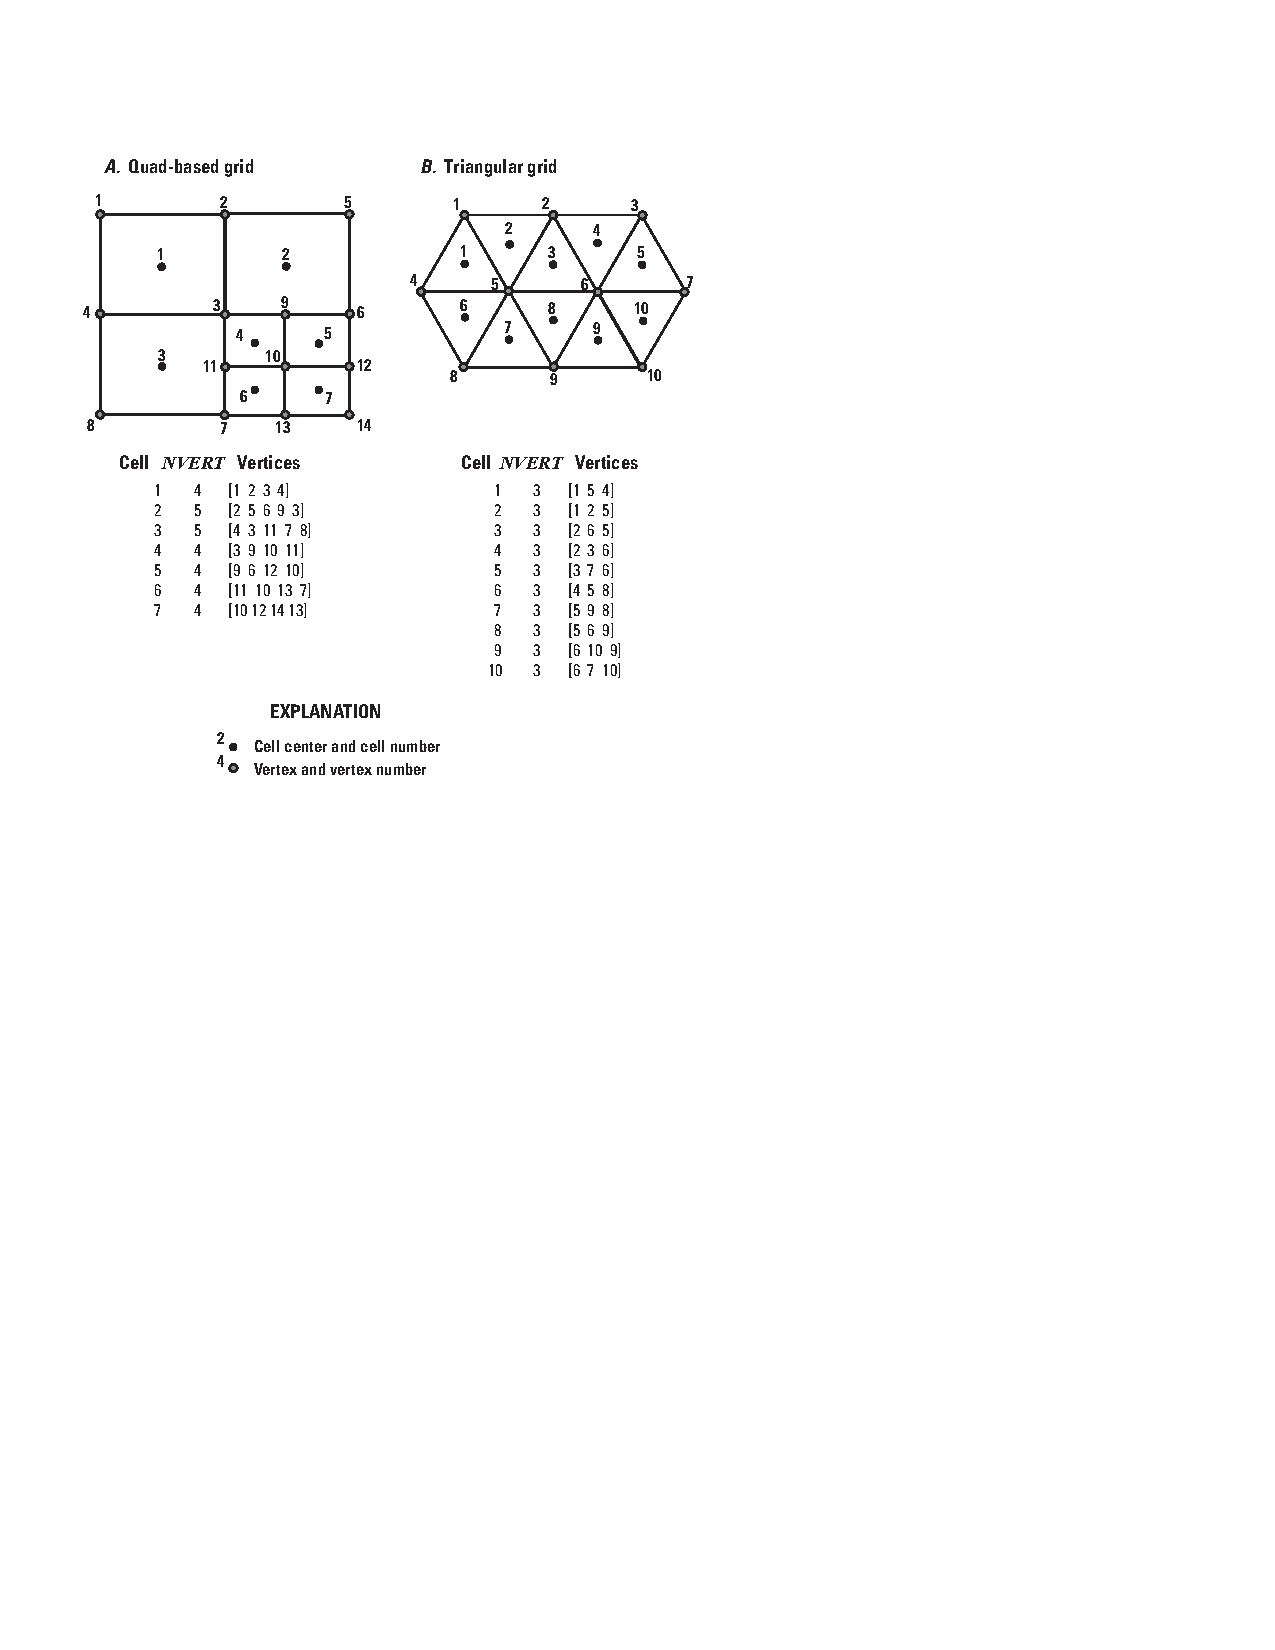
\includegraphics[scale=1.0]{Figures/gwf-fig3-2}
	\caption{Schematic diagram showing the vertices and cells defined using the Discretization by Vertices Package. The list of vertices used to define each cell must be in clockwise order.  From \cite{modflow6gwf}}
	\label{fig:gwf-fig3-2}
\end{figure}


\vspace{5mm}
\subsubsection{Structure of Blocks}
\lstinputlisting[style=blockdefinition]{./mf6ivar/tex/gwf-disv-options.dat}
\lstinputlisting[style=blockdefinition]{./mf6ivar/tex/gwf-disv-dimensions.dat}
\lstinputlisting[style=blockdefinition]{./mf6ivar/tex/gwf-disv-griddata.dat}
\lstinputlisting[style=blockdefinition]{./mf6ivar/tex/gwf-disv-vertices.dat}
\lstinputlisting[style=blockdefinition]{./mf6ivar/tex/gwf-disv-cell2d.dat}

\vspace{5mm}
\subsubsection{Explanation of Variables}
\begin{description}
\input{./mf6ivar/tex/gwf-disv-desc.tex}
\end{description}

\vspace{5mm}
\subsubsection{Example Input File}
\lstinputlisting[style=inputfile]{./mf6ivar/examples/gwf-disv-example.dat}


%\newpage
%\subsection{Unstructured Discretization (DISU) Input File}
%Discretization information for unstructured grids is read from the file that is specified by ``DISU6'' as the file type.  Only one discretization input file (DISU6, DISV6 or DIS6) can be specified for a model.

The shape and position of each cell can be defined using vertices.  This information is optional and is only read if the number of vertices (NVERT) in the DIMENSIONS block is specified and is assigned a value larger than zero.  If the vertices and two-dimensional cell information is provided in this file, then this information is also written to the binary grid file.  Providing this information may be useful for other postprocessing programs that read the binary grid file.

The DISU Package does not support the concept of layers, which is different from the DISU implementation in MODFLOW-USG.  In \mf~all grid input and output for models that use the DISU Package is entered or written as a one-dimensional array of size nodes.

The DISU VERTICES and CELL2D blocks are not required for all simulations.  These blocks are required if the XT3D or the SAVE\_SPECIFIC\_DISCHARGE options are specified in the NPF Package.  In general, it is recommended to include the VERTICES and CELL2D blocks. 

\vspace{5mm}
\subsubsection{Structure of Blocks}
\lstinputlisting[style=blockdefinition]{./mf6ivar/tex/gwf-disu-options.dat}
\lstinputlisting[style=blockdefinition]{./mf6ivar/tex/gwf-disu-dimensions.dat}
\lstinputlisting[style=blockdefinition]{./mf6ivar/tex/gwf-disu-griddata.dat}
\lstinputlisting[style=blockdefinition]{./mf6ivar/tex/gwf-disu-connectiondata.dat}
\lstinputlisting[style=blockdefinition]{./mf6ivar/tex/gwf-disu-vertices.dat}
\lstinputlisting[style=blockdefinition]{./mf6ivar/tex/gwf-disu-cell2d.dat}

\vspace{5mm}
\subsubsection{Explanation of Variables}
\begin{description}
\input{./mf6ivar/tex/gwf-disu-desc.tex}
\end{description}

\vspace{5mm}
\subsubsection{Example Input File}
\lstinputlisting[style=inputfile]{./mf6ivar/examples/gwf-disu-example.dat}



\newpage
\subsection{Initial Conditions (IC) Package}
Initial Conditions (IC) Package information is read from the file that is specified by ``IC6'' as the file type.  Only one IC Package can be specified for a GWE model. 

\vspace{5mm}
\subsubsection{Structure of Blocks}
\lstinputlisting[style=blockdefinition]{./mf6ivar/tex/gwe-ic-options.dat}
\lstinputlisting[style=blockdefinition]{./mf6ivar/tex/gwe-ic-griddata.dat}

\vspace{5mm}
\subsubsection{Explanation of Variables}
\begin{description}
\input{./mf6ivar/tex/gwe-ic-desc.tex}
\end{description}

\vspace{5mm}
\subsubsection{Example Input File}
\lstinputlisting[style=inputfile]{./mf6ivar/examples/gwe-ic-example.dat}



\newpage
\subsection{Output Control (OC) Option}
Input to the Output Control Option of the Surface Water Flow Model is read from the file that is specified as type ``OC6'' in the Name File. If no ``OC6'' file is specified, default output control is used. The Output Control Option determines how and when outflows are printed to the listing file and/or written to a separate binary output file.  Under the default, outflow and overall flow budget are written to the Listing File at the end of every stress period. The default printout format for concentrations is 10G11.4.  The outflow and overall flow budget are also written to the list file if the simulation terminates prematurely due to failed convergence.

\vspace{5mm}
\subsubsection{Structure of Blocks}
\vspace{5mm}

\noindent \textit{FOR EACH SIMULATION}
\lstinputlisting[style=blockdefinition]{./mf6ivar/tex/olf-oc-options.dat}
\vspace{5mm}
\noindent \textit{FOR ANY STRESS PERIOD}
\lstinputlisting[style=blockdefinition]{./mf6ivar/tex/olf-oc-period.dat}

\vspace{5mm}
\subsubsection{Explanation of Variables}
\begin{description}
\input{./mf6ivar/tex/olf-oc-desc.tex}
\end{description}

\vspace{5mm}
\subsubsection{Example Input File}
\lstinputlisting[style=inputfile]{./mf6ivar/examples/olf-oc-example.dat}


\newpage
\subsection{Observation (OBS) Utility for a GWT Model}

GWT Model observations include the simulated groundwater concentration (\texttt{concentration}), and the mass flow, with units of mass per time, between two connected cells (\texttt{flow-ja-face}). The data required for each GWT Model observation type is defined in table~\ref{table:gwtobstype}. For \texttt{flow-ja-face} observation types, negative and positive values represent a loss from and gain to the \texttt{cellid} specified for ID, respectively.

\subsubsection{Structure of Blocks}
\vspace{5mm}

\noindent \textit{FOR EACH SIMULATION}
\lstinputlisting[style=blockdefinition]{./mf6ivar/tex/utl-obs-options.dat}
\lstinputlisting[style=blockdefinition]{./mf6ivar/tex/utl-obs-continuous.dat}

\subsubsection{Explanation of Variables}
\begin{description}
\input{./mf6ivar/tex/utl-obs-desc.tex}
\end{description}


\begin{longtable}{p{2cm} p{2.75cm} p{2cm} p{1.25cm} p{7cm}}
\caption{Available GWT model observation types} \tabularnewline

\hline
\hline
\textbf{Model} & \textbf{Observation type} & \textbf{ID} & \textbf{ID2} & \textbf{Description} \\
\hline
\endhead

\hline
\endfoot


GWT Model observations include the simulated groundwater concentration (\texttt{concentration}), and the mass flow, with units of mass per time, between two connected cells (\texttt{flow-ja-face}). The data required for each GWT Model observation type is defined in table~\ref{table:gwtobstype}. For \texttt{flow-ja-face} observation types, negative and positive values represent a loss from and gain to the \texttt{cellid} specified for ID, respectively.

\subsubsection{Structure of Blocks}
\vspace{5mm}

\noindent \textit{FOR EACH SIMULATION}
\lstinputlisting[style=blockdefinition]{./mf6ivar/tex/utl-obs-options.dat}
\lstinputlisting[style=blockdefinition]{./mf6ivar/tex/utl-obs-continuous.dat}

\subsubsection{Explanation of Variables}
\begin{description}
\input{./mf6ivar/tex/utl-obs-desc.tex}
\end{description}


\begin{longtable}{p{2cm} p{2.75cm} p{2cm} p{1.25cm} p{7cm}}
\caption{Available GWT model observation types} \tabularnewline

\hline
\hline
\textbf{Model} & \textbf{Observation type} & \textbf{ID} & \textbf{ID2} & \textbf{Description} \\
\hline
\endhead

\hline
\endfoot


GWT Model observations include the simulated groundwater concentration (\texttt{concentration}), and the mass flow, with units of mass per time, between two connected cells (\texttt{flow-ja-face}). The data required for each GWT Model observation type is defined in table~\ref{table:gwtobstype}. For \texttt{flow-ja-face} observation types, negative and positive values represent a loss from and gain to the \texttt{cellid} specified for ID, respectively.

\subsubsection{Structure of Blocks}
\vspace{5mm}

\noindent \textit{FOR EACH SIMULATION}
\lstinputlisting[style=blockdefinition]{./mf6ivar/tex/utl-obs-options.dat}
\lstinputlisting[style=blockdefinition]{./mf6ivar/tex/utl-obs-continuous.dat}

\subsubsection{Explanation of Variables}
\begin{description}
\input{./mf6ivar/tex/utl-obs-desc.tex}
\end{description}


\begin{longtable}{p{2cm} p{2.75cm} p{2cm} p{1.25cm} p{7cm}}
\caption{Available GWT model observation types} \tabularnewline

\hline
\hline
\textbf{Model} & \textbf{Observation type} & \textbf{ID} & \textbf{ID2} & \textbf{Description} \\
\hline
\endhead

\hline
\endfoot

\input{../Common/gwt-obs.tex}
\label{table:gwtobstype}
\end{longtable}

\vspace{5mm}
\subsubsection{Example Observation Input File}

An example GWT Model observation file is shown below.

\lstinputlisting[style=inputfile]{./mf6ivar/examples/utl-obs-gwt-example.dat}


\label{table:gwtobstype}
\end{longtable}

\vspace{5mm}
\subsubsection{Example Observation Input File}

An example GWT Model observation file is shown below.

\lstinputlisting[style=inputfile]{./mf6ivar/examples/utl-obs-gwt-example.dat}


\label{table:gwtobstype}
\end{longtable}

\vspace{5mm}
\subsubsection{Example Observation Input File}

An example GWT Model observation file is shown below.

\lstinputlisting[style=inputfile]{./mf6ivar/examples/utl-obs-gwt-example.dat}



\newpage
\subsection{Advection (ADV) Package}
Advection (ADV) Package information is read from the file that is specified by ``ADV6'' as the file type.  Only one ADV Package can be specified for a GWT model. 

\vspace{5mm}
\subsubsection{Structure of Blocks}
\lstinputlisting[style=blockdefinition]{./mf6ivar/tex/gwt-adv-options.dat}

\vspace{5mm}
\subsubsection{Explanation of Variables}
\begin{description}
\input{./mf6ivar/tex/gwt-adv-desc.tex}
\end{description}

\vspace{5mm}
\subsubsection{Example Input File}
\lstinputlisting[style=inputfile]{./mf6ivar/examples/gwt-adv-example.dat}



\newpage
\subsection{Dispersion (DSP) Package}
Dispersion (DSP) Package information is read from the file that is specified by ``DSP6'' as the file type.  Only one DSP Package can be specified for a GWT model.  By default, the DSP Package uses the mathematical formulation presented for the XT3D option of the NPF Package to represent full three-dimensional anisotropy in groundwater flow.  XT3D can be computationally expensive and can be turned off to use a simplified and approximate form of the dispersion equations.  For most problems, however, XT3D will be required to accurately represent dispersion.

\vspace{5mm}
\subsubsection{Structure of Blocks}
\lstinputlisting[style=blockdefinition]{./mf6ivar/tex/gwt-dsp-options.dat}
\lstinputlisting[style=blockdefinition]{./mf6ivar/tex/gwt-dsp-griddata.dat}

\vspace{5mm}
\subsubsection{Explanation of Variables}
\begin{description}
\input{./mf6ivar/tex/gwt-dsp-desc.tex}
\end{description}

\vspace{5mm}
\subsubsection{Example Input File}
\lstinputlisting[style=inputfile]{./mf6ivar/examples/gwt-dsp-example.dat}



\newpage
\subsection{Source and Sink Mixing (SSM) Package}
Source and Sink Mixing (SSM) Package information is read from the file that is specified by ``SSM6'' as the file type.  Only one SSM Package can be specified for a GWT model.  The SSM Package is required if the flow model has any stress packages.

The SSM Package is used to add or remove solute mass from GWT model cells based on inflows and outflows from GWF stress packages.  If a GWF stress package provides flow into a model cell, that flow can be assigned a user-specified concentration.  If a GWT stress package removes water from a model cell, the concentration of that water is typically the concentration of the cell, but a ``MIXED'' option is also included so that the user can specify the concentration of that withdrawn water.  This may be useful for representing evapotranspiration, for example.  There are several different ways for the user to specify the concentrations.  

\begin{itemize}
\item The default condition is that sources have a concentration of zero and sinks withdraw water at the calculated concentration of the cell.  This default condition is assigned to any GWF stress package that is not included in a SOURCES block or FILEINPUT block.
\item A second option is to assign auxiliary variables in the GWF model and include a concentration for each stress boundary.  In this case, the user provides the name of the package and the name of the auxiliary variable containing concentration values for each boundary.  As described below for srctype, there are multiple options for defining this behavior.
\item  A third option is to prepare an input file using the \hyperref[sec:spc]{Stress Package Component (SPC6) utility} for any desired GWF stress package.  This SPC6 file allows users to change concentrations by stress period, or to use the time-series option to interpolate concentrations by time step.  This third option was introduced in MODFLOW version 6.3.0.  Information for this approach is entered in an optional FILEINPUT block below.  The SPC6 input file supports list-based concentration input for most corresponding GWF stress packages, but also supports a READASARRAYS array-based input format if a corresponding GWF recharge or evapotranspiration package uses the READASARRAYS option.
\end{itemize}

\noindent The auxiliary method and the SPC6 file input method can both be used for a GWT model, but only one approach can be assigned per GWF stress package.   If a flow package specified in the SOURCES or FILEINPUT blocks is also represented using an advanced transport package (SFT, LKT, MWT, or UZT), then the advanced transport package will override SSM calculations for that package.

\vspace{5mm}
\subsubsection{Structure of Blocks}
\lstinputlisting[style=blockdefinition]{./mf6ivar/tex/gwt-ssm-options.dat}
\lstinputlisting[style=blockdefinition]{./mf6ivar/tex/gwt-ssm-sources.dat}
\vspace{5mm}
\noindent \textit{FILEINPUT BLOCK IS OPTIONAL}
\lstinputlisting[style=blockdefinition]{./mf6ivar/tex/gwt-ssm-fileinput.dat}

\vspace{5mm}
\subsubsection{Explanation of Variables}
\begin{description}
\input{./mf6ivar/tex/gwt-ssm-desc.tex}
\end{description}

\vspace{5mm}
\subsubsection{Example Input File}
\lstinputlisting[style=inputfile]{./mf6ivar/examples/gwt-ssm-example.dat}

% when obs are ready, they should go here


\newpage
\subsection{Mobile Storage and Transfer (MST) Package}
Mobile Storage and Transfer (MST) Package information is read from the file that is specified by ``MST6'' as the file type.  Only one MST Package can be specified for a GWT model. 

\vspace{5mm}
\subsubsection{Structure of Blocks}
\lstinputlisting[style=blockdefinition]{./mf6ivar/tex/gwt-mst-options.dat}
\lstinputlisting[style=blockdefinition]{./mf6ivar/tex/gwt-mst-griddata.dat}

\vspace{5mm}
\subsubsection{Explanation of Variables}
\begin{description}
\input{./mf6ivar/tex/gwt-mst-desc.tex}
\end{description}

\vspace{5mm}
\subsubsection{Example Input File}
\lstinputlisting[style=inputfile]{./mf6ivar/examples/gwt-mst-example.dat}



\newpage
\subsection{Immobile Storage and Transfer (IST) Package}
Immobile Storage and Transfer (IST) Package information is read from the file that is specified by ``IST6'' as the file type.  Any number of IST Packages can be specified for a single GWT model.  This allows the user to specify triple porosity systems, or systems with as many immobile domains as necessary. 

Subsequent to MODFLOW Version 6.4.1, substantial changes were made to the input parameter definitions and conceptualization of the IST Package.  These changes are described in Chapter 9 of the MODFLOW 6 Supplemental Technical Information document that is included with the distribution.

\vspace{5mm}
\subsubsection{Structure of Blocks}
\lstinputlisting[style=blockdefinition]{./mf6ivar/tex/gwt-ist-options.dat}
\lstinputlisting[style=blockdefinition]{./mf6ivar/tex/gwt-ist-griddata.dat}

\vspace{5mm}
\subsubsection{Explanation of Variables}
\begin{description}
\input{./mf6ivar/tex/gwt-ist-desc.tex}
\end{description}

\vspace{5mm}
\subsubsection{Example Input File}
\lstinputlisting[style=inputfile]{./mf6ivar/examples/gwt-ist-example.dat}



\newpage
\subsection{Constant Concentration (CNC) Package}
Constant Concentration (CNC) Package information is read from the file that is specified by ``CNC6'' as the file type.  Any number of CNC Packages can be specified for a single GWT model, but the same cell cannot be designated as a constant concentration by more than one CNC entry. 

\vspace{5mm}
\subsubsection{Structure of Blocks}
\vspace{5mm}

\noindent \textit{FOR EACH SIMULATION}
\lstinputlisting[style=blockdefinition]{./mf6ivar/tex/gwt-cnc-options.dat}
\lstinputlisting[style=blockdefinition]{./mf6ivar/tex/gwt-cnc-dimensions.dat}
\vspace{5mm}
\noindent \textit{FOR ANY STRESS PERIOD}
\lstinputlisting[style=blockdefinition]{./mf6ivar/tex/gwt-cnc-period.dat}
\packageperioddescription

\vspace{5mm}
\subsubsection{Explanation of Variables}
\begin{description}
\input{./mf6ivar/tex/gwt-cnc-desc.tex}
\end{description}

\vspace{5mm}
\subsubsection{Example Input File}
\lstinputlisting[style=inputfile]{./mf6ivar/examples/gwt-cnc-example.dat}

\vspace{5mm}
\subsubsection{Available observation types}
CNC Package observations are limited to the simulated constant concentration mass flow rate (\texttt{cnc}). The data required for the CNC Package observation type is defined in table~\ref{table:gwt-cncobstype}. Negative and positive values for an observation represent a loss from and gain to the GWT model, respectively.

\begin{longtable}{p{2cm} p{2.75cm} p{2cm} p{1.25cm} p{7cm}}
\caption{Available CNC Package observation types} \tabularnewline

\hline
\hline
\textbf{Model} & \textbf{Observation type} & \textbf{ID} & \textbf{ID2} & \textbf{Description} \\
\hline
\endhead

\hline
\endfoot

CNC & cnc & cellid or boundname & -- & Mass flow between the groundwater system and a constant-concentration boundary or a group of cells with constant-concentration boundaries.

\label{table:gwt-cncobstype}
\end{longtable}

\vspace{5mm}
\subsubsection{Example Observation Input File}
\lstinputlisting[style=inputfile]{./mf6ivar/examples/gwt-cnc-example-obs.dat}


\newpage
\subsection{Mass Source Loading (SRC) Package}
Input to the Mass Source Loading (SRC) Package is read from the file that has type ``SRC6'' in the Name File.  Any number of SRC Packages can be specified for a single groundwater transport model.

\vspace{5mm}
\subsubsection{Structure of Blocks}
\vspace{5mm}

\noindent \textit{FOR EACH SIMULATION}
\lstinputlisting[style=blockdefinition]{./mf6ivar/tex/gwt-src-options.dat}
\lstinputlisting[style=blockdefinition]{./mf6ivar/tex/gwt-src-dimensions.dat}
\vspace{5mm}
\noindent \textit{FOR ANY STRESS PERIOD}
\lstinputlisting[style=blockdefinition]{./mf6ivar/tex/gwt-src-period.dat}
\packageperioddescription

\vspace{5mm}
\subsubsection{Explanation of Variables}
\begin{description}
\input{./mf6ivar/tex/gwt-src-desc.tex}
\end{description}

\vspace{5mm}
\subsubsection{Example Input File}
\lstinputlisting[style=inputfile]{./mf6ivar/examples/gwt-src-example.dat}

\vspace{5mm}
\subsubsection{Available observation types}
Mass Source Loading Package observations include the simulated source loading rates (\texttt{src}). The data required for each SRC Package observation type is defined in table~\ref{table:gwt-srcobstype}. The \texttt{src} observation is equal to the simulated mass source loading rate. Negative and positive values for an observation represent a loss from and gain to the GWT model, respectively.

\begin{longtable}{p{2cm} p{2.75cm} p{2cm} p{1.25cm} p{7cm}}
\caption{Available SRC Package observation types} \tabularnewline

\hline
\hline
\textbf{Stress Package} & \textbf{Observation type} & \textbf{ID} & \textbf{ID2} & \textbf{Description} \\
\hline
\endhead

\hline
\endfoot

SRC & src & cellid or boundname & -- & Mass source loading rate between the groundwater system and a mass source loading boundary or a group of  boundaries.
\label{table:gwt-srcobstype}
\end{longtable}

\vspace{5mm}
\subsubsection{Example Observation Input File}
\lstinputlisting[style=inputfile]{./mf6ivar/examples/gwt-src-example-obs.dat}


\newpage
\subsection{Streamflow Transport (SFT) Package}
Streamflow Transport (SFT) Package information is read from the file that is specified by ``SFT6'' as the file type.  There can be as many SFT Packages as necessary for a GWT model. Each SFT Package is designed to work with flows from a corresponding GWF SFR Package. By default \mf uses the SFT package name to determine which SFR Package corresponds to the SFT Package.  Therefore, the package name of the SFT Package (as specified in the GWT name file) must match with the name of the corresponding SFR Package (as specified in the GWF name file).  Alternatively, the name of the flow package can be specified using the FLOW\_PACKAGE\_NAME keyword in the options block.  The GWT SFT Package cannot be used without a corresponding GWF SFR Package.

The SFT Package does not have a dimensions block; instead, dimensions for the SFT Package are set using the dimensions from the corresponding SFR Package.  For example, the SFR Package requires specification of the number of reaches (NREACHES).  SFT sets the number of reaches equal to NREACHES.  Therefore, the PACKAGEDATA block below must have NREACHES entries in it.

\vspace{5mm}
\subsubsection{Structure of Blocks}
\lstinputlisting[style=blockdefinition]{./mf6ivar/tex/gwt-sft-options.dat}
\lstinputlisting[style=blockdefinition]{./mf6ivar/tex/gwt-sft-packagedata.dat}
\lstinputlisting[style=blockdefinition]{./mf6ivar/tex/gwt-sft-period.dat}

\vspace{5mm}
\subsubsection{Explanation of Variables}
\begin{description}
\input{./mf6ivar/tex/gwt-sft-desc.tex}
\end{description}

\vspace{5mm}
\subsubsection{Example Input File}
\lstinputlisting[style=inputfile]{./mf6ivar/examples/gwt-sft-example.dat}

\vspace{5mm}
\subsubsection{Available observation types}
Streamflow Transport Package observations include reach concentration and all of the terms that contribute to the continuity equation for each reach. Additional SFT Package observations include mass flow rates for individual reaches, or groups of reaches. The data required for each SFT Package observation type is defined in table~\ref{table:gwt-sftobstype}. Negative and positive values for \texttt{sft} observations represent a loss from and gain to the GWT model, respectively. For all other flow terms, negative and positive values represent a loss from and gain from the SFT package, respectively.

\begin{longtable}{p{2cm} p{2.75cm} p{2cm} p{1.25cm} p{7cm}}
\caption{Available SFT Package observation types} \tabularnewline

\hline
\hline
\textbf{Stress Package} & \textbf{Observation type} & \textbf{ID} & \textbf{ID2} & \textbf{Description} \\
\hline
\endfirsthead

\captionsetup{textformat=simple}
\caption*{\textbf{Table \arabic{table}.}{\quad}Available SFT Package observation types.---Continued} \tabularnewline

\hline
\hline
\textbf{Stress Package} & \textbf{Observation type} & \textbf{ID} & \textbf{ID2} & \textbf{Description} \\
\hline
\endhead


\hline
\endfoot

% general APT observations
SFT & concentration & ifno or boundname & -- & Reach concentration. If boundname is specified, boundname must be unique for each reach. \\
SFT & flow-ja-face & ifno or boundname & ifno or -- & Mass flow between two reaches.  If a boundname is specified for ID1, then the result is the total mass flow for all reaches. If a boundname is specified for ID1 then ID2 is not used.\\
SFT & storage & ifno or boundname & -- & Simulated mass storage flow rate for a reach or group of reaches. \\
SFT & constant & ifno or boundname & -- & Simulated mass constant-flow rate for a reach or group of reaches. \\
SFT & from-mvr & ifno or boundname & -- & Simulated mass inflow into a reach or group of reaches from the MVT package. Mass inflow is calculated as the product of provider concentration and the mover flow rate. \\
SFT & to-mvr & ifno or boundname & -- & Mass outflow from a reach, or a group of reaches that is available for the MVR package. If boundname is not specified for ID, then the outflow available for the MVR package from a specific reach is observed. \\
SFT & sft & ifno or boundname & -- & Mass flow rate for a reach or group of reaches and its aquifer connection(s). \\

%observations specific to the stream transport package
% rainfall evaporation runoff ext-inflow withdrawal outflow
SFT & rainfall & ifno or boundname & -- & Rainfall rate applied to a reach or group of reaches multiplied by the rainfall concentration. \\
SFT & evaporation & ifno or boundname & -- & Simulated evaporation rate from a reach or group of reaches multiplied by the evaporation concentration. \\
SFT & runoff & ifno or boundname & -- & Runoff rate applied to a reach or group of reaches multiplied by the runoff concentration. \\
SFT & ext-inflow & ifno or boundname & -- & Mass inflow into a reach or group of reaches calculated as the external inflow rate multiplied by the inflow concentration. \\
SFT & ext-outflow & ifno or boundname & -- & External outflow from a reach or group of reaches to an external boundary. If boundname is not specified for ID, then the external outflow from a specific reach is observed. In this case, ID is the reach ifno.

\label{table:gwt-sftobstype}
\end{longtable}

\vspace{5mm}
\subsubsection{Example Observation Input File}
\lstinputlisting[style=inputfile]{./mf6ivar/examples/gwt-sft-example-obs.dat}




\newpage
\subsection{Lake Transport (LKT) Package}
Lake Transport (LKT) Package information is read from the file that is specified by ``LKT6'' as the file type.  There can be as many LKT Packages as necessary for a GWT model. Each LKT Package is designed to work with flows from a single corresponding GWF LAK Package. By default \mf uses the LKT package name to determine which LAK Package corresponds to the LKT Package.  Therefore, the package name of the LKT Package (as specified in the GWT name file) must match with the name of the corresponding LAK Package (as specified in the GWF name file).  Alternatively, the name of the flow package can be specified using the FLOW\_PACKAGE\_NAME keyword in the options block.  The GWT LKT Package cannot be used without a corresponding GWF LAK Package.

The LKT Package does not have a dimensions block; instead, dimensions for the LKT Package are set using the dimensions from the corresponding LAK Package.  For example, the LAK Package requires specification of the number of lakes (NLAKES).  LKT sets the number of lakes equal to NLAKES.  Therefore, the PACKAGEDATA block below must have NLAKES entries in it.

\vspace{5mm}
\subsubsection{Structure of Blocks}
\lstinputlisting[style=blockdefinition]{./mf6ivar/tex/gwt-lkt-options.dat}
\lstinputlisting[style=blockdefinition]{./mf6ivar/tex/gwt-lkt-packagedata.dat}
\lstinputlisting[style=blockdefinition]{./mf6ivar/tex/gwt-lkt-period.dat}

\vspace{5mm}
\subsubsection{Explanation of Variables}
\begin{description}
\input{./mf6ivar/tex/gwt-lkt-desc.tex}
\end{description}

\vspace{5mm}
\subsubsection{Example Input File}
\lstinputlisting[style=inputfile]{./mf6ivar/examples/gwt-lkt-example.dat}

\vspace{5mm}
\subsubsection{Available observation types}
Lake Transport Package observations include lake concentration and all of the terms that contribute to the continuity equation for each lake. Additional LKT Package observations include mass flow rates for individual outlets, lakes, or groups of lakes (\texttt{outlet}). The data required for each LKT Package observation type is defined in table~\ref{table:gwt-lktobstype}. Negative and positive values for \texttt{lkt} observations represent a loss from and gain to the GWT model, respectively. For all other flow terms, negative and positive values represent a loss from and gain from the LKT package, respectively.

\begin{longtable}{p{2cm} p{2.75cm} p{2cm} p{1.25cm} p{7cm}}
\caption{Available LKT Package observation types} \tabularnewline

\hline
\hline
\textbf{Stress Package} & \textbf{Observation type} & \textbf{ID} & \textbf{ID2} & \textbf{Description} \\
\hline
\endfirsthead

\captionsetup{textformat=simple}
\caption*{\textbf{Table \arabic{table}.}{\quad}Available LKT Package observation types.---Continued} \tabularnewline

\hline
\hline
\textbf{Stress Package} & \textbf{Observation type} & \textbf{ID} & \textbf{ID2} & \textbf{Description} \\
\hline
\endhead


\hline
\endfoot

% general APT observations
LKT & concentration & ifno or boundname & -- & Lake concentration. If boundname is specified, boundname must be unique for each lake. \\
LKT & flow-ja-face & ifno or boundname & ifno or -- & Mass flow between two lakes connected by an outlet.  If more than one outlet is used to connect the same two lakes, then the mass flow for only the first outlet can be observed.  If a boundname is specified for ID1, then the result is the total mass flow for all outlets for a lake. If a boundname is specified for ID1 then ID2 is not used.\\
LKT & storage & ifno or boundname & -- & Simulated mass storage flow rate for a lake or group of lakes. \\
LKT & constant & ifno or boundname & -- & Simulated mass constant-flow rate for a lake or group of lakes. \\
LKT & from-mvr & ifno or boundname & -- & Simulated mass inflow into a lake or group of lakes from the MVT package. Mass inflow is calculated as the product of provider concentration and the mover flow rate. \\
LKT & to-mvr & outletno or boundname & -- & Mass outflow from a lake outlet, a lake, or a group of lakes that is available for the MVR package. If boundname is not specified for ID, then the outflow available for the MVR package from a specific lake outlet is observed. In this case, ID is the outlet number, which must be between 1 and NOUTLETS. \\
LKT & lkt & ifno or boundname & \texttt{iconn} or -- & Mass flow rate for a lake or group of lakes and its aquifer connection(s). If boundname is not specified for ID, then the simulated lake-aquifer flow rate at a specific lake connection is observed. In this case, ID2 must be specified and is the connection number \texttt{iconn} for lake \texttt{ifno}. \\

%observations specific to the lake package
% rainfall evaporation runoff ext-inflow withdrawal outflow
LKT & rainfall & ifno or boundname & -- & Rainfall rate applied to a lake or group of lakes multiplied by the rainfall concentration. \\
LKT & evaporation & ifno or boundname & -- & Simulated evaporation rate from a lake or group of lakes multiplied by the evaporation concentration. \\
LKT & runoff & ifno or boundname & -- & Runoff rate applied to a lake or group of lakes multiplied by the runoff concentration. \\
LKT & ext-inflow & ifno or boundname & -- & Mass inflow into a lake or group of lakes calculated as the external inflow rate multiplied by the inflow concentration. \\
LKT & withdrawal & ifno or boundname & -- & Specified withdrawal rate from a lake or group of lakes multiplied by the simulated lake concentration. \\
LKT & ext-outflow & ifno or boundname & -- & External outflow from a lake or a group of lakes, through their outlets, to an external boundary.  If the water mover is active, the reported ext-outflow value plus the rate to mover is equal to the total outlet outflow.

%LKT & outlet-inflow & ifno or boundname & -- & Simulated inflow from upstream lake outlets into a lake or group of lakes. \\
%LKT & inflow & ifno or boundname & -- & Sum of specified inflow and simulated inflow from upstream lake outlets into a lake or group of lakes. \\
%LKT & outlet & outletno or boundname & -- & Simulate outlet flow rate from a lake outlet, a lake, or a group of lakes. If boundname is not specified for ID, then the flow from a specific lake outlet is observed. In this case, ID is the outlet number outletno. \\
%LKT & volume & ifno or boundname & -- & Simulated lake volume or group of lakes. \\
%LKT & surface-area & ifno or boundname & -- & Simulated surface area for a lake or group of lakes. \\
%LKT & wetted-area & ifno or boundname & \texttt{iconn} or -- & Simulated wetted-area for a lake or group of lakes and its aquifer connection(s). If boundname is not specified for ID, then the wetted area of a specific lake connection is observed. In this case, ID2 must be specified and is the connection number \texttt{iconn}. \\
%LKT & conductance & ifno or boundname & \texttt{iconn} or -- & Calculated conductance for a lake or group of lakes and its aquifer connection(s). If boundname is not specified for ID, then the calculated conductance of a specific lake connection is observed. In this case, ID2 must be specified and is the connection number \texttt{iconn}.

\label{table:gwt-lktobstype}
\end{longtable}

\vspace{5mm}
\subsubsection{Example Observation Input File}
\lstinputlisting[style=inputfile]{./mf6ivar/examples/gwt-lkt-example-obs.dat}




\newpage
\subsection{Multi-Aquifer Well Transport (MWT) Package}
Multi-Aquifer Well Transport (MWT) Package information is read from the file that is specified by ``MWT6'' as the file type.  There can be as many MWT Packages as necessary for a GWT model. Each MWT Package is designed to work with flows from a corresponding GWF MAW Package. By default \mf uses the MWT package name to determine which MAW Package corresponds to the MWT Package.  Therefore, the package name of the MWT Package (as specified in the GWT name file) must match with the name of the corresponding MAW Package (as specified in the GWF name file).  Alternatively, the name of the flow package can be specified using the FLOW\_PACKAGE\_NAME keyword in the options block.  The GWT MWT Package cannot be used without a corresponding GWF MAW Package.

The MWT Package does not have a dimensions block; instead, dimensions for the MWT Package are set using the dimensions from the corresponding MAW Package.  For example, the MAW Package requires specification of the number of wells (NMAWWELLS).  MWT sets the number of wells equal to NMAWWELLS.  Therefore, the PACKAGEDATA block below must have NMAWWELLS entries in it.

\vspace{5mm}
\subsubsection{Structure of Blocks}
\lstinputlisting[style=blockdefinition]{./mf6ivar/tex/gwt-mwt-options.dat}
\lstinputlisting[style=blockdefinition]{./mf6ivar/tex/gwt-mwt-packagedata.dat}
\lstinputlisting[style=blockdefinition]{./mf6ivar/tex/gwt-mwt-period.dat}

\vspace{5mm}
\subsubsection{Explanation of Variables}
\begin{description}
\input{./mf6ivar/tex/gwt-mwt-desc.tex}
\end{description}

\vspace{5mm}
\subsubsection{Example Input File}
\lstinputlisting[style=inputfile]{./mf6ivar/examples/gwt-mwt-example.dat}

\vspace{5mm}
\subsubsection{Available observation types}
Multi-Aquifer Well Transport Package observations include well concentration and all of the terms that contribute to the continuity equation for each well. Additional MWT Package observations include mass flow rates for individual wells, or groups of wells; the well volume (\texttt{volume}); and the conductance for a well-aquifer connection conductance (\texttt{conductance}). The data required for each MWT Package observation type is defined in table~\ref{table:gwt-mwtobstype}. Negative and positive values for \texttt{mwt} observations represent a loss from and gain to the GWT model, respectively. For all other flow terms, negative and positive values represent a loss from and gain from the MWT package, respectively.

\begin{longtable}{p{2cm} p{2.75cm} p{2cm} p{1.25cm} p{7cm}}
\caption{Available MWT Package observation types} \tabularnewline

\hline
\hline
\textbf{Stress Package} & \textbf{Observation type} & \textbf{ID} & \textbf{ID2} & \textbf{Description} \\
\hline
\endfirsthead

\captionsetup{textformat=simple}
\caption*{\textbf{Table \arabic{table}.}{\quad}Available MWT Package observation types.---Continued} \tabularnewline

\hline
\hline
\textbf{Stress Package} & \textbf{Observation type} & \textbf{ID} & \textbf{ID2} & \textbf{Description} \\
\hline
\endhead


\hline
\endfoot

% general APT observations
MWT & concentration & ifno or boundname & -- & Well concentration. If boundname is specified, boundname must be unique for each well. \\
%flowjaface not included
MWT & storage & ifno or boundname & -- & Simulated mass storage flow rate for a well or group of wells. \\
MWT & constant & ifno or boundname & -- & Simulated mass constant-flow rate for a well or group of wells. \\
MWT & from-mvr & ifno or boundname & -- & Simulated mass inflow into a well or group of wells from the MVT package. Mass inflow is calculated as the product of provider concentration and the mover flow rate. \\
MWT & mwt & ifno or boundname & \texttt{iconn} or -- & Mass flow rate for a well or group of wells and its aquifer connection(s). If boundname is not specified for ID, then the simulated well-aquifer flow rate at a specific well connection is observed. In this case, ID2 must be specified and is the connection number \texttt{iconn} for well \texttt{ifno}. \\

% observations specific to the mwt package
MWT & rate & ifno or boundname & -- & Simulated mass flow rate for a well or group of wells. \\
MWT & fw-rate & ifno or boundname & -- & Simulated mass flow rate for a flowing well or group of flowing wells. \\
MWT & rate-to-mvr & well or boundname & -- & Simulated mass flow rate that is sent to the MVT Package for a well or group of wells.\\
MWT & fw-rate-to-mvr & well or boundname & -- & Simulated mass flow rate that is sent to the MVT Package from a flowing well or group of flowing wells. \\

\label{table:gwt-mwtobstype}
\end{longtable}

\vspace{5mm}
\subsubsection{Example Observation Input File}
\lstinputlisting[style=inputfile]{./mf6ivar/examples/gwt-mwt-example-obs.dat}




\newpage
\subsection{Unsaturated Zone Transport (UZT) Package}
Unsaturated Zone Transport (UZT) Package information is read from the file that is specified by ``UZT6'' as the file type.  There can be as many UZT Packages as necessary for a GWT model. Each UZT Package is designed to work with flows from a corresponding GWF UZF Package. By default \mf uses the UZT package name to determine which UZF Package corresponds to the UZT Package.  Therefore, the package name of the UZT Package (as specified in the GWT name file) must match with the name of the corresponding UZF Package (as specified in the GWF name file).  Alternatively, the name of the flow package can be specified using the FLOW\_PACKAGE\_NAME keyword in the options block.  The GWT UZT Package cannot be used without a corresponding GWF UZF Package.

The UZT Package does not have a dimensions block; instead, dimensions for the UZT Package are set using the dimensions from the corresponding UZF Package.  For example, the UZF Package requires specification of the number of cells (NUZFCELLS).  UZT sets the number of UZT cells equal to NUZFCELLS.  Therefore, the PACKAGEDATA block below must have NUZFCELLS entries in it.

\vspace{5mm}
\subsubsection{Structure of Blocks}
\lstinputlisting[style=blockdefinition]{./mf6ivar/tex/gwt-uzt-options.dat}
\lstinputlisting[style=blockdefinition]{./mf6ivar/tex/gwt-uzt-packagedata.dat}
\lstinputlisting[style=blockdefinition]{./mf6ivar/tex/gwt-uzt-period.dat}

\vspace{5mm}
\subsubsection{Explanation of Variables}
\begin{description}
\input{./mf6ivar/tex/gwt-uzt-desc.tex}
\end{description}

\vspace{5mm}
\subsubsection{Example Input File}
\lstinputlisting[style=inputfile]{./mf6ivar/examples/gwt-uzt-example.dat}

\vspace{5mm}
\subsubsection{Available observation types}
Unsaturated Zone Transport Package observations include UZF cell concentration and all of the terms that contribute to the continuity equation for each UZF cell. Additional UZT Package observations include mass flow rates for individual UZF cells, or groups of UZF cells. The data required for each UZT Package observation type is defined in table~\ref{table:gwt-uztobstype}. Negative and positive values for \texttt{uzt} observations represent a loss from and gain to the GWT model, respectively. For all other flow terms, negative and positive values represent a loss from and gain from the UZT package, respectively.

\begin{longtable}{p{2cm} p{2.75cm} p{2cm} p{1.25cm} p{7cm}}
\caption{Available UZT Package observation types} \tabularnewline

\hline
\hline
\textbf{Stress Package} & \textbf{Observation type} & \textbf{ID} & \textbf{ID2} & \textbf{Description} \\
\hline
\endfirsthead

\captionsetup{textformat=simple}
\caption*{\textbf{Table \arabic{table}.}{\quad}Available UZT Package observation types.---Continued} \tabularnewline

\hline
\hline
\textbf{Stress Package} & \textbf{Observation type} & \textbf{ID} & \textbf{ID2} & \textbf{Description} \\
\hline
\endhead


\hline
\endfoot

% general APT observations
UZT & concentration & ifno or boundname & -- & uzt cell concentration. If boundname is specified, boundname must be unique for each uzt cell. \\
UZT & flow-ja-face & ifno or boundname & ifno or -- & Mass flow between two uzt cells.  If a boundname is specified for ID1, then the result is the total mass flow for all uzt cells. If a boundname is specified for ID1 then ID2 is not used.\\
UZT & storage & ifno or boundname & -- & Simulated mass storage flow rate for a uzt cell or group of uzt cells. \\
UZT & constant & ifno or boundname & -- & Simulated mass constant-flow rate for a uzt cell or a group of uzt cells. \\
UZT & from-mvr & ifno or boundname & -- & Simulated mass inflow into a uzt cell or group of uzt cells from the MVT package. Mass inflow is calculated as the product of provider concentration and the mover flow rate. \\
UZT & uzt & ifno or boundname & -- & Mass flow rate for a uzt cell or group of uzt cells and its aquifer connection(s). \\

%observations specific to the uzt package
% infiltration rej-inf uzet rej-inf-to-mvr
UZT & infiltration & ifno or boundname & -- & Infiltration rate applied to a uzt cell or group of uzt cells multiplied by the infiltration concentration. \\
UZT & rej-inf & ifno or boundname & -- & Rejected infiltration rate applied to a uzt cell or group of uzt cells multiplied by the infiltration concentration. \\
UZT & uzet & ifno or boundname & -- & Unsaturated zone evapotranspiration rate applied to a uzt cell or group of uzt cells multiplied by the uzt cell concentration. \\
UZT & rej-inf-to-mvr & ifno or boundname & -- & Rejected infiltration rate applied to a uzt cell or group of uzt cells multiplied by the infiltration concentration that is sent to the mover package. \\

\label{table:gwt-uztobstype}
\end{longtable}

\vspace{5mm}
\subsubsection{Example Observation Input File}
\lstinputlisting[style=inputfile]{./mf6ivar/examples/gwt-uzt-example-obs.dat}




\newpage
\subsection{Flow Model Interface (FMI) Package}
Flow Model Interface (FMI) Package information is read from the file that is specified by ``FMI6'' as the file type.  The FMI Package file is required only if the PRT Model is running in a separate simulation from a previously run GWF Model. If the PRT Model is coupled to a GWF Model by an exchange, the FMI Package file is not required. Only one FMI Package can be specified for a PRT model.

The PRT Model needs groundwater flows for model grid cells, for boundary conditions, and for other terms, such as the flow of water in or out of storage.  The FMI Package is the interface between the PRT Model and simulated groundwater flows provided by a corresponding GWF Model that is running concurrently within the simulation or from binary budget files that were created from a previous GWF model run.  The following are several different FMI simulation cases:

\begin{itemize}

\item Flows are provided by a corresponding GWF Model running in the same simulation---in this case, all groundwater flows are calculated by the corresponding GWF Model and provided through FMI to the transport model.  This is a common use case in which the user wants to run the flow and particle-tracking models as part of a single simulation.  The GWF and PRT models must be part of a GWF-PRT Exchange that is listed in mfsim.nam.  If a GWF-PRT Exchange is specified by the user, then the user does not need to specify an FMI Package input file for the simulation, unless an FMI option is needed.  If a GWF-PRT Exchange is specified and the FMI Package is specified, then the PACKAGEDATA block below is not read or used.

\item Flows are provided from a previous GWF model simulation---in this case FMI should be provided in the PRT name file and the head and budget files should be listed in the FMI PACKAGEDATA block.  In this case, FMI reads the simulated head and flows from these files and makes them available to the particle-tracking model.  There are some additional considerations when the heads and flows are provided from binary files.

\begin{itemize}
\item The binary budget file must contain the simulated flows for all of the packages that were included in the GWF model run.  Saving of flows can be activated for all packages by specifying ``SAVE\_FLOWS'' as an option in the GWF name file.  The GWF Output Control Package must also have ``SAVE BUDGET ALL'' specified.  The easiest way to ensure that all flows and heads are saved is to use the following simple form of a GWF Output Control file:

\begin{verbatim}
BEGIN OPTIONS
  HEAD FILEOUT mymodel.hds
  BUDGET FILEOUT mymodel.bud
END OPTIONS

BEGIN PERIOD 1
  SAVE HEAD ALL
  SAVE BUDGET ALL
END PERIOD
\end{verbatim}

\item The binary budget file must have the same number of budget terms listed for each time step.  This will always be the case when the binary budget file is created by \mf.
\item The binary heads file must have heads saved for all layers in the model.  This will always be the case when the binary head file is created by \mf.  This was not always the case as previous MODFLOW versions allowed different save options for each layer.
\item If the binary budget and head files have more than one time step for a single stress period, then the budget and head information must be contained within the binary file for every time step in the simulation stress period.
\item The binary budget and head files must correspond in terms of information stored for each time step and stress period.
\item If the binary budget and head files have information provided for only the first time step of a given stress period, this information will be used for all time steps in that stress period in the PRT simulation. If the final (or only) stress period in the binary budget and head files contains data for only one time step, this information will be used for any subsequent time steps and stress periods in the PRT simulation. This makes it possible to provide flows, for example, from a steady-state GWF stress period and have those flows used for all PRT time steps in that stress period, for all remaining time steps in the PRT simulation, or for all time steps throughout the entire PRT simulation. With this option, it is possible to have smaller time steps in the PRT simulation than the time steps used in the GWF simulation. Note that this cannot be done when the GWF and PRT models are run in the same simulation, because in that case, both models are solved over the same sequence of time steps and stress periods, as listed in the TDIS Package. The option to read flows from a previous GWF simulation via Flow Model Interface may offer an efficient alternative to running both models in the same simulation, but comes at the cost of having potentially very large budget files.
\item The binary grid file is optional but recommended, as it allows \mf to verify that the GWF and PRT model grids are identical.
\end{itemize}

\end{itemize}

\noindent Determination of which FMI use case to invoke requires careful consideration of the different advantages and disadvantages of each case.  For example, running PRT and GWF in the same simulation can often be faster because GWF flows are passed through memory to the PRT model instead of being written to files.  The disadvantage of this approach is that the same time step lengths must be used for both GWF and PRT.  Ultimately, it should be relatively straightforward to test different ways in which GWF and PRT interact and select the use case most appropriate for the particular problem. 

\vspace{5mm}
\subsubsection{Structure of Blocks}
\lstinputlisting[style=blockdefinition]{./mf6ivar/tex/prt-fmi-packagedata.dat}

\vspace{5mm}
\subsubsection{Explanation of Variables}
\begin{description}
\input{./mf6ivar/tex/prt-fmi-desc.tex}
\end{description}

\vspace{5mm}
\subsubsection{Example Input File}
\lstinputlisting[style=inputfile]{./mf6ivar/examples/prt-fmi-example.dat}



\newpage
\subsection{Mover Transport (MVT) Package}
Mover Transport (MVT) Package information is read from the file that is specified by ``MVT6'' as the file type.  Only one MVT Package can be specified for a GWT model.  

The MVT Package is used to route solute mass according to flows from the GWF Water Mover (MVR) Package.  This MVT Package must be activated by the user if the MVR Package was active for the GWF Model.  Flows from the GWF MVR Package must be available to the GWT model either through activation of a GWF-GWT Exchange or through specification of ``GWFMOVER'' in the PACKAGEDATA block of the GWT FMI Package.  

\vspace{5mm}
\subsubsection{Structure of Blocks}
\lstinputlisting[style=blockdefinition]{./mf6ivar/tex/gwt-mvt-options.dat}

\vspace{5mm}
\subsubsection{Explanation of Variables}
\begin{description}
\input{./mf6ivar/tex/gwt-mvt-desc.tex}
\end{description}

\vspace{5mm}
\subsubsection{Example Input File}
\lstinputlisting[style=inputfile]{./mf6ivar/examples/gwt-mvt-example.dat}



\newpage
\subsection{Groundwater Transport (GWT) Exchange}
Input to the Groundwater Transport (GWT-GWT) Exchange is read from the file that has type ``GWT6-GWT6'' in the Simulation Name File.

The list of exchanges entered into the EXCHANGEDATA block must be identical to the list of exchanges entered for the GWF-GWF input file.  One way to ensure that this information is identical is to put this list into an external file and refer to this same list using the OPEN/CLOSE functionality in both this EXCHANGEDATA input block and the EXCHANGEDATA input block in the GWF-GWF input file.

\vspace{5mm}
\subsubsection{Structure of Blocks}
\lstinputlisting[style=blockdefinition]{./mf6ivar/tex/exg-gwtgwt-options.dat}
\lstinputlisting[style=blockdefinition]{./mf6ivar/tex/exg-gwtgwt-dimensions.dat}
\lstinputlisting[style=blockdefinition]{./mf6ivar/tex/exg-gwtgwt-exchangedata.dat}

\vspace{5mm}
\subsubsection{Explanation of Variables}
\begin{description}
\input{./mf6ivar/tex/exg-gwtgwt-desc.tex}
\end{description}

\vspace{5mm}
\subsubsection{Example Input File}
\lstinputlisting[style=inputfile]{./mf6ivar/examples/exg-gwtgwt-example.dat}

\vspace{5mm}
\subsubsection{Available observation types}
GWT-GWT Exchange observations include the simulated flow for any exchange (\texttt{flow-ja-face}). The data required for each GWT-GWT Exchange observation type is defined in table~\ref{table:gwt-gwtobstype}. For \texttt{flow-ja-face} observation types, negative and positive values represent a loss from and gain to the first model specified for this exchange.

\begin{longtable}{p{2cm} p{2.75cm} p{2cm} p{1.25cm} p{7cm}}
\caption{Available GWT-GWT Exchange observation types} \tabularnewline

\hline
\hline
\textbf{Exchange} & \textbf{Observation type} & \textbf{ID} & \textbf{ID2} & \textbf{Description} \\
\hline
\endhead

\hline
\endfoot

GWT-GWT & flow-ja-face & exchange number or boundname & -- & Mass flow between model 1 and model 2 for a specified exchange (which is the consecutive exchange number listed in the EXCHANGEDATA block), or the sum of these exchange flows by boundname if boundname is specified.
\label{table:gwt-gwtobstype}
\end{longtable}


\vspace{5mm}
\subsubsection{Example Observation Input File}
\lstinputlisting[style=inputfile]{./mf6ivar/examples/exg-gwtgwt-example-obs.dat}



